\documentclass[a4paper,11pt]{article}

\usepackage[utf8]{inputenc}
\title{ARC2 -- TP 7}
\author{Prune Forget, Léo Noël-Baron \& Thierry Sampaio}
\date{16/03/2016}

\usepackage{a4wide}
\usepackage{textcomp}
\usepackage[utf8]{inputenc}
\usepackage[T1]{fontenc}
\usepackage[francais]{babel}

\usepackage{graphicx}
\usepackage[usenames,dvipsnames]{color}

\usepackage{hyperref} \urlstyle{sf}
\hypersetup{
  colorlinks=true,
  urlcolor=BlueViolet,
  citecolor=BlueViolet,
  linkcolor=BlueViolet,
}
\DeclareUrlCommand\email{\urlstyle{sf}}

\newenvironment{keywords}
  {\description\item[\bsc{Mots-clés}]~$\cdot$~ }
  {\enddescription}
\newenvironment{remarque}
  {\description\item[\bsc{Remarque} ---]\sl}
  {\enddescription}
\renewcommand{\thefootnote}{\arabic{footnote}}

\usepackage{listings}
\lstset{
  language=C,
  basicstyle=\ttfamily,
  keywordstyle=\color{OliveGreen},
  stringstyle=\color{Bittersweet},
  showstringspaces=false,
  commentstyle=\color{Gray},
  numbers=left,
  numberstyle=\ttfamily\color{Gray},
  frame=l,
  columns=fullflexible,
  rulecolor=\color{Gray},
  tabsize=4,
  extendedchars=true,
  literate=
	{É}{{\'E}}1 {è}{{\`e}}1 {à}{{\`a}}1 {È}{{\`E}}1 {À}{{\`A}}1 {ê}{{\^e}}1 {â}{{\^a}}1 {î}{{\^\i}}1 {ô}{{\^o}}1
	{Ê}{{\^E}}1 {Â}{{\^A}}1 {Î}{{\^I}}1 {Ô}{{\^O}}1 {Û}{{\^U}}1 {ë}{{\"e}}1 {ï}{{\"\i}}1 {ü}{{\"u}}1 {Ë}{{\"E}}1
	{Ï}{{\"I}}1 {Ü}{{\"U}}1 {û}{{\^u}}1 {ç}{{\c c}}1 {Ç}{{\c C}}1 {æ}{{\ae}}1 {Æ}{{\AE}}1 {œ}{{\oe}}1 {Œ}{{\OE}}1
	{é}{{\'e}}1,
}
\lstMakeShortInline{|}

\parskip=0.3\baselineskip
\sloppy

\makeatletter
  \let\runtitle\@title
  \let\runauthor\@author
\makeatother

\usepackage{fancyhdr}
\pagestyle{fancy}
\fancyhead{}
\lhead{\runtitle}
\rhead{\runauthor}
\setlength{\headheight}{13.6pt}


\begin{document}

\maketitle

Ce TP propose de gérer un clavier d'entrée sur le BihaNios.

\subsection*{Connexions au bus}

On choisit d'utiliser pour l'entrée les interrupteurs \verb?SW[14..7]?, que l'on doit rediriger sur le \verb?Bus[7..0]? si l'adresse demandée est 0x8000. L'adressage se fait donc en conjuguant \verb?Lec? et \verb?MA[31]?, comme exposé en figure \ref{async}.

\begin{figure}[h]\center
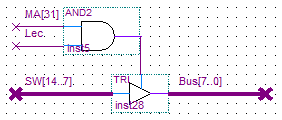
\includegraphics[scale=0.7]{tp7-1.PNG}
\caption{Interface sans synchronisation}
\label{async}
\end{figure}

\subsection*{Programme de test}

Voici le programme utilisé pour tester l'interface de base :
\begin{lstlisting}[language=Lisp]
.equ AddLec 0x8000
debut:
            addi r6,r0,0 ; Initialisation
while:
			; Lecture de l'entrée clavier dans r9
            ldw r9,AddLec(r0)
            andi r9,r9,0xFF ; Masque pour prendre seulement 8 bits
            ; Sommation et affichage
            add r6,r6,r9
            stw r6,1024(r0)
            br while
            
.end debut
\end{lstlisting}

En exécutant le programme pas à pas, on peut basculer l'entrée à 0 une fois qu'elle a été interprétée. En continu, cela devient impossible et les nombres s'additionnent anarchiquement.

\subsection*{Interface avec bit d'état}

On réalise un bit d'état au moyen de deux portes NOR (R en haut, S en bas) ; le bouton \verb?NKEY[2]? doit le mettre à 1 et il doit être lu dans \verb?Bus[0]? à l'adresse 0x8001, c'est-à-dire quand \verb?Lec ^ MA[15] ^ MA[0]?. Il doit être remis à 0 soit manuellement par le bouton \verb?NKEY[0]?, soit après lecture de l'entrée (on reprend donc le signal de lecture précédent, en tenant compte cette fois de \verb?MA[0]?). On obtient le circuit en Figure \ref{sync}.

\begin{figure}[h]\center
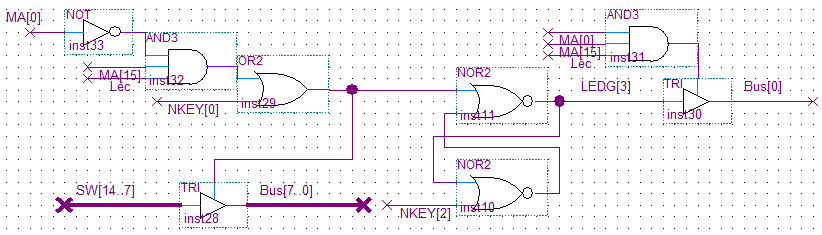
\includegraphics[scale=0.7]{tp7-2.PNG}
\caption{Interface avec synchronisation}
\label{sync}
\end{figure}

On a maintenant un bit d'état activé manuellement pour signaler qu'un entrée est prête, qui se désactive lorsque l'entrée a été lue. Ceci permet de modifier le programme précédent pour y rajouter une attente active sur ce bit d'état :
\begin{lstlisting}[language=Lisp]
.equ AddLec 0x8000
.equ State 0x8001 ; Bit d'état
debut:
            addi r6,r0,0
while:
            ; On commence par charger le bit d'état
            ldw r9,State(r0)
            andi r9,r9,0x1 ; Masque sur le bit de poids faible
            ; S'il n'y a rien à lire, on boucle directement
            beq r9,r0,while
            ; Sinon, on lit l'entrée et on l'interprète comme avant
            ldw r9,AddLec(r0)
            andi r9,r9,0xFF
            add r6,r6,r9
            stw r6,1024(r0)
            br while
            
.end debut
\end{lstlisting}

Le programme se comporte maintenant comme on le souhaite ; chaque entrée n'est lue qu'une seule fois, lorsque la frappe est signalée.

\end{document}
